\documentclass{standalone}
\usepackage{tikz}
\usetikzlibrary{patterns, positioning}
\usepackage[sfdefault]{ClearSans} %% option 'sfdefault' activates Clear Sans as the default text font
\usepackage[T1]{fontenc}

\begin{document}
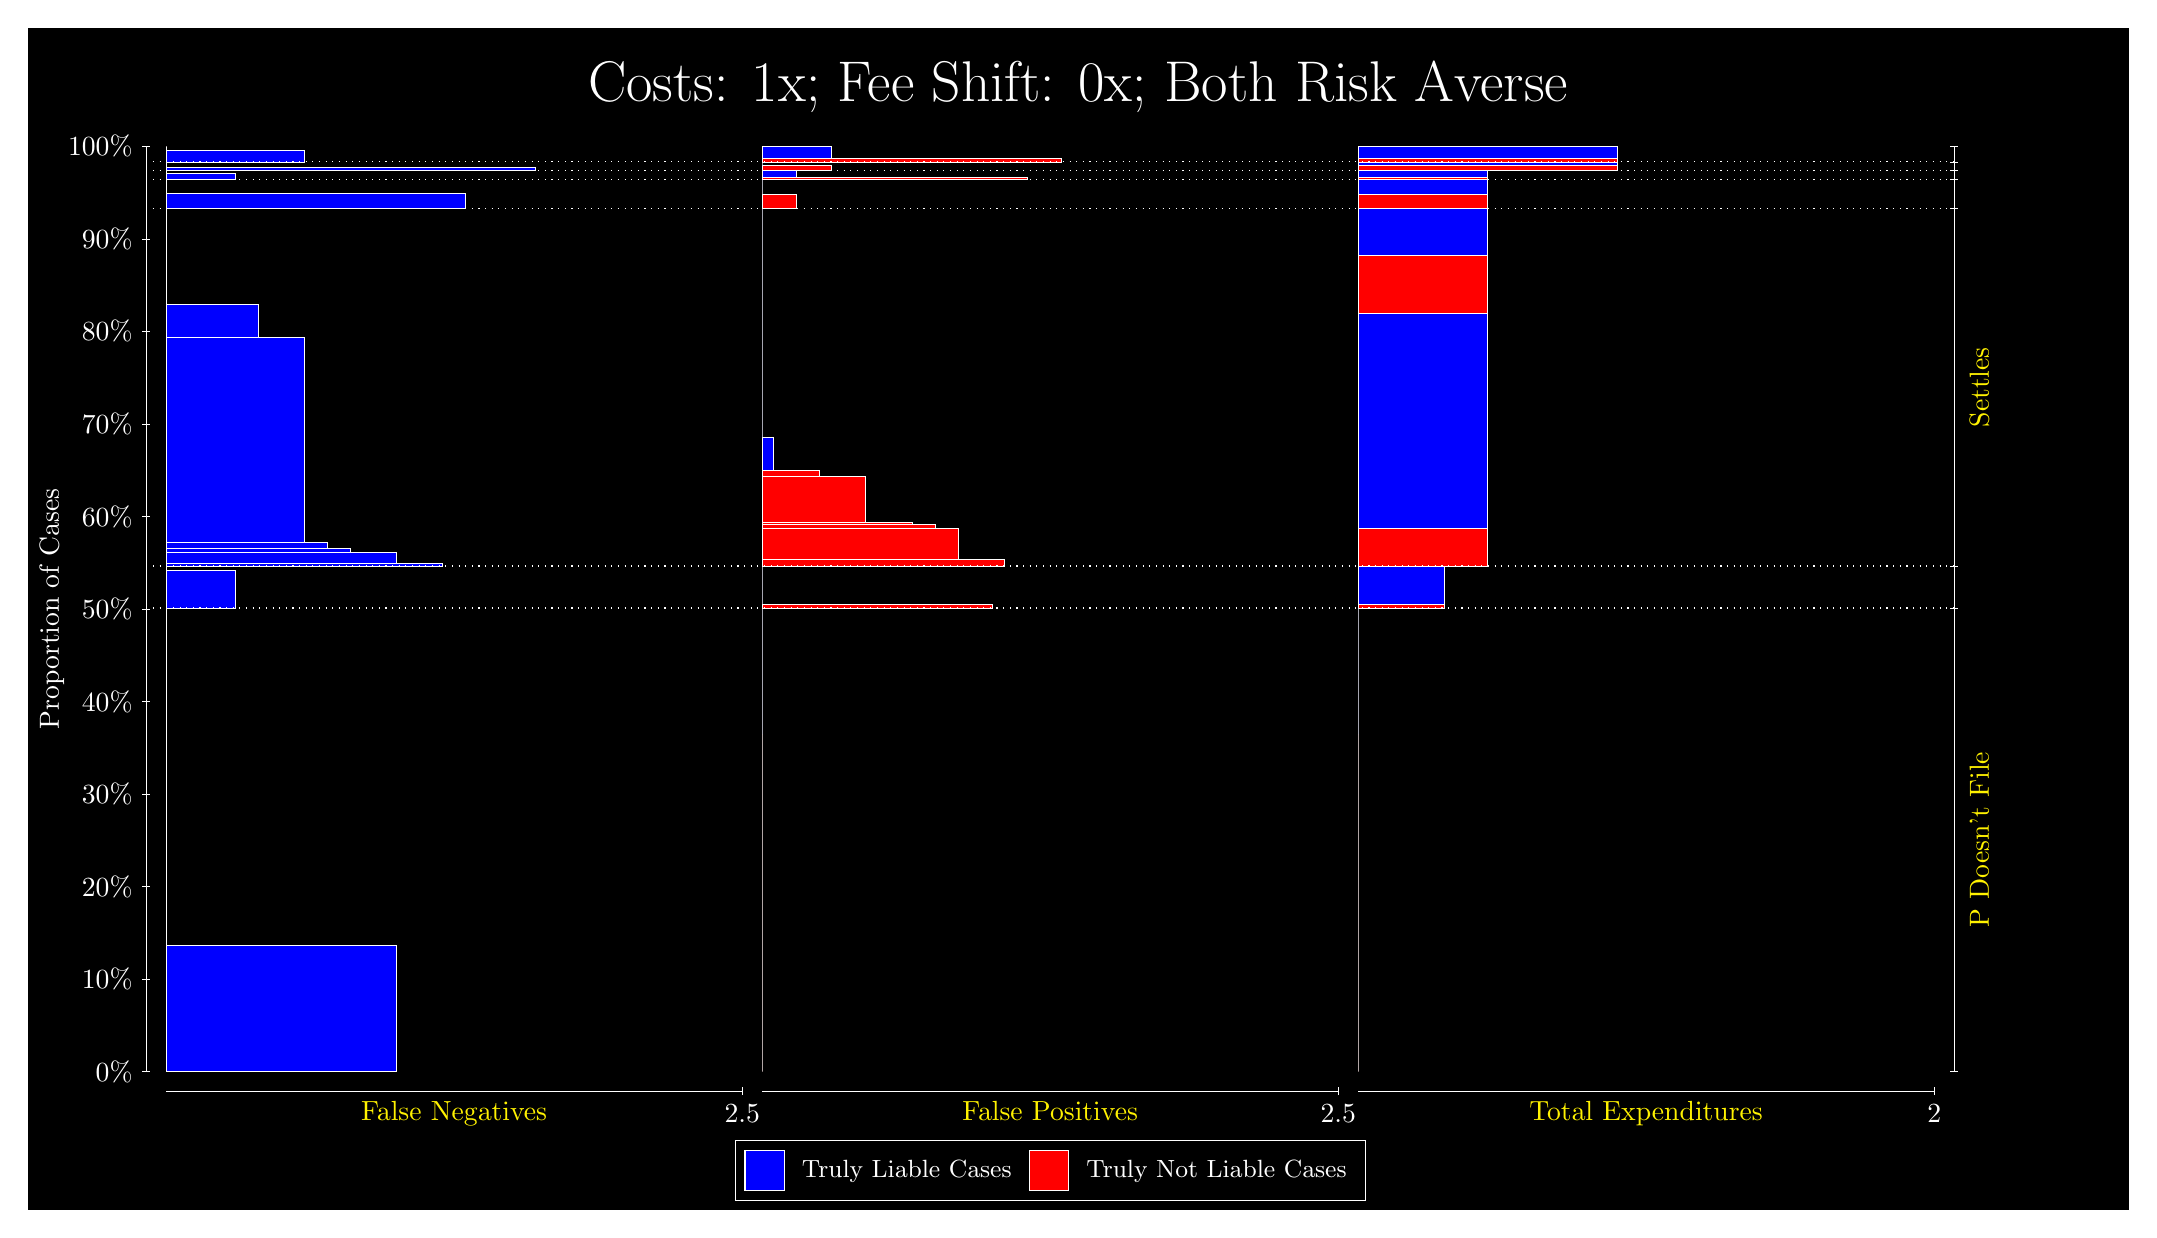
\begin{tikzpicture}
\draw[fill=black] (0,0) rectangle (26.667,15);
\draw[text=white] (0,13.5) rectangle (26.667,15) node[midway] {\huge Costs: 1x; Fee Shift: 0x; Both Risk Averse};
\draw[white, very thin] (1.5,1.75) -- (1.5,13.5);
\node[rotate=90, text=white, anchor=center] at (0.3, 7.625) {Proportion of Cases};
\draw[white, very thin] (1.45,1.75) -- (1.55,1.75);
\node[text=white, anchor=east] at (1.45, 1.75) {0\%};
\draw[white, very thin] (1.45,2.925) -- (1.55,2.925);
\node[text=white, anchor=east] at (1.45, 2.925) {10\%};
\draw[white, very thin] (1.45,4.1) -- (1.55,4.1);
\node[text=white, anchor=east] at (1.45, 4.1) {20\%};
\draw[white, very thin] (1.45,5.275) -- (1.55,5.275);
\node[text=white, anchor=east] at (1.45, 5.275) {30\%};
\draw[white, very thin] (1.45,6.45) -- (1.55,6.45);
\node[text=white, anchor=east] at (1.45, 6.45) {40\%};
\draw[white, very thin] (1.45,7.625) -- (1.55,7.625);
\node[text=white, anchor=east] at (1.45, 7.625) {50\%};
\draw[white, very thin] (1.45,8.8) -- (1.55,8.8);
\node[text=white, anchor=east] at (1.45, 8.8) {60\%};
\draw[white, very thin] (1.45,9.975) -- (1.55,9.975);
\node[text=white, anchor=east] at (1.45, 9.975) {70\%};
\draw[white, very thin] (1.45,11.15) -- (1.55,11.15);
\node[text=white, anchor=east] at (1.45, 11.15) {80\%};
\draw[white, very thin] (1.45,12.325) -- (1.55,12.325);
\node[text=white, anchor=east] at (1.45, 12.325) {90\%};
\draw[white, very thin] (1.45,13.5) -- (1.55,13.5);
\node[text=white, anchor=east] at (1.45, 13.5) {100\%};

\draw[white, very thin] (24.457,1.75) -- (24.457,13.5);
\draw[white, very thin] (24.407,1.75) -- (24.507,1.75);
\node[anchor=west] at (24.407, 1.75) {};
\draw[white, very thin] (24.407,7.6364) -- (24.507,7.6364);
\node[anchor=west] at (24.407, 7.6364) {};
\draw[white, very thin] (24.407,8.1702) -- (24.507,8.1702);
\node[anchor=west] at (24.407, 8.1702) {};
\draw[white, very thin] (24.407,12.711) -- (24.507,12.711);
\node[anchor=west] at (24.407, 12.711) {};
\draw[white, very thin] (24.407,13.083) -- (24.507,13.083);
\node[anchor=west] at (24.407, 13.083) {};
\draw[white, very thin] (24.407,13.192) -- (24.507,13.192);
\node[anchor=west] at (24.407, 13.192) {};
\draw[white, very thin] (24.407,13.303) -- (24.507,13.303);
\node[anchor=west] at (24.407, 13.303) {};
\draw[white, very thin] (24.407,13.5) -- (24.507,13.5);
\node[anchor=west] at (24.407, 13.5) {};

\draw[white, very thin, fill=blue] (1.75,1.75) rectangle (4.6775,3.35);
\draw[white, very thin, fill=red] (1.75,3.35) rectangle (1.75,7.6364);
\draw[white, very thin, fill=blue] (1.75,7.6364) rectangle (2.6283,8.117);
\draw[white, very thin, fill=red] (1.75,8.117) rectangle (1.75,8.1702);
\draw[white, very thin, fill=blue] (1.75,8.1702) rectangle (5.2631,8.202);
\draw[white, very thin, fill=blue] (1.75,8.202) rectangle (4.6775,8.3433);
\draw[white, very thin, fill=blue] (1.75,8.3433) rectangle (4.092,8.3995);
\draw[white, very thin, fill=blue] (1.75,8.3995) rectangle (3.7993,8.4656);
\draw[white, very thin, fill=blue] (1.75,8.4656) rectangle (3.5065,11.081);
\draw[white, very thin, fill=blue] (1.75,11.081) rectangle (2.921,11.5);
\draw[white, very thin, fill=red] (1.75,11.5) rectangle (1.75,12.711);
\draw[white, very thin, fill=blue] (1.75,12.711) rectangle (5.5558,12.898);
\draw[white, very thin, fill=red] (1.75,12.898) rectangle (1.75,13.083);
\draw[white, very thin, fill=blue] (1.75,13.083) rectangle (2.6283,13.164);
\draw[white, very thin, fill=red] (1.75,13.164) rectangle (1.75,13.192);
\draw[white, very thin, fill=blue] (1.75,13.192) rectangle (6.4341,13.24);
\draw[white, very thin, fill=red] (1.75,13.24) rectangle (1.75,13.303);
\draw[white, very thin, fill=blue] (1.75,13.303) rectangle (3.5065,13.452);
\draw[white, very thin, fill=red] (1.75,13.452) rectangle (1.75,13.5);
\draw[white, very thin, fill=red] (9.3189,1.75) rectangle (9.3189,6.0364);
\draw[white, very thin, fill=blue] (9.3189,6.0364) rectangle (9.3189,7.6364);
\draw[white, very thin, fill=red] (9.3189,7.6364) rectangle (12.246,7.6896);
\draw[white, very thin, fill=blue] (9.3189,7.6896) rectangle (9.3189,8.1702);
\draw[white, very thin, fill=red] (9.3189,8.1702) rectangle (12.393,8.2555);
\draw[white, very thin, fill=red] (9.3189,8.2555) rectangle (11.807,8.6504);
\draw[white, very thin, fill=red] (9.3189,8.6504) rectangle (11.515,8.6949);
\draw[white, very thin, fill=red] (9.3189,8.6949) rectangle (11.222,8.7314);
\draw[white, very thin, fill=red] (9.3189,8.7314) rectangle (10.636,9.3091);
\draw[white, very thin, fill=red] (9.3189,9.3091) rectangle (10.051,9.3811);
\draw[white, very thin, fill=blue] (9.3189,9.3811) rectangle (9.4652,9.8004);
\draw[white, very thin, fill=blue] (9.3189,9.8004) rectangle (9.3189,12.711);
\draw[white, very thin, fill=red] (9.3189,12.711) rectangle (9.758,12.896);
\draw[white, very thin, fill=blue] (9.3189,12.896) rectangle (9.3189,13.083);
\draw[white, very thin, fill=red] (9.3189,13.083) rectangle (12.686,13.111);
\draw[white, very thin, fill=blue] (9.3189,13.111) rectangle (9.758,13.192);
\draw[white, very thin, fill=red] (9.3189,13.192) rectangle (10.197,13.255);
\draw[white, very thin, fill=blue] (9.3189,13.255) rectangle (9.3189,13.303);
\draw[white, very thin, fill=red] (9.3189,13.303) rectangle (13.125,13.352);
\draw[white, very thin, fill=blue] (9.3189,13.352) rectangle (10.197,13.5);
\draw[white, very thin, fill=red] (16.888,1.75) rectangle (16.888,6.0364);
\draw[white, very thin, fill=blue] (16.888,6.0364) rectangle (16.888,7.6364);
\draw[white, very thin, fill=red] (16.888,7.6364) rectangle (17.986,7.6896);
\draw[white, very thin, fill=blue] (16.888,7.6896) rectangle (17.986,8.1702);
\draw[white, very thin, fill=red] (16.888,8.1702) rectangle (18.534,8.6461);
\draw[white, very thin, fill=blue] (16.888,8.6461) rectangle (18.534,11.384);
\draw[white, very thin, fill=red] (16.888,11.384) rectangle (18.534,12.119);
\draw[white, very thin, fill=blue] (16.888,12.119) rectangle (18.534,12.711);
\draw[white, very thin, fill=red] (16.888,12.711) rectangle (18.534,12.896);
\draw[white, very thin, fill=blue] (16.888,12.896) rectangle (18.534,13.083);
\draw[white, very thin, fill=red] (16.888,13.083) rectangle (18.534,13.111);
\draw[white, very thin, fill=blue] (16.888,13.111) rectangle (18.534,13.192);
\draw[white, very thin, fill=red] (16.888,13.192) rectangle (20.181,13.255);
\draw[white, very thin, fill=blue] (16.888,13.255) rectangle (20.181,13.303);
\draw[white, very thin, fill=red] (16.888,13.303) rectangle (20.181,13.352);
\draw[white, very thin, fill=blue] (16.888,13.352) rectangle (20.181,13.5);
\draw[white, dotted] (1.5,7.6364) -- (24.457,7.6364);
\draw[white, dotted] (1.5,8.1702) -- (24.457,8.1702);
\draw[white, dotted] (1.5,12.711) -- (24.457,12.711);
\draw[white, dotted] (1.5,13.083) -- (24.457,13.083);
\draw[white, dotted] (1.5,13.192) -- (24.457,13.192);
\draw[white, dotted] (1.5,13.303) -- (24.457,13.303);
\draw[white, very thin] (1.75,1.5) -- (9.0689,1.5);
\node[text=yellow, anchor=north] at (5.4094, 1.5) {False Negatives};
\draw[white, very thin] (9.0689,1.45) -- (9.0689,1.55);
\node[text=white, anchor=north] at (9.0689, 1.45) {2.5};

\draw[white, very thin] (9.3189,1.5) -- (16.638,1.5);
\node[text=yellow, anchor=north] at (12.978, 1.5) {False Positives};
\draw[white, very thin] (16.638,1.45) -- (16.638,1.55);
\node[text=white, anchor=north] at (16.638, 1.45) {2.5};

\draw[white, very thin] (16.888,1.5) -- (24.207,1.5);
\node[text=yellow, anchor=north] at (20.547, 1.5) {Total Expenditures};
\draw[white, very thin] (24.207,1.45) -- (24.207,1.55);
\node[text=white, anchor=north] at (24.207, 1.45) {2};

\node[text=yellow, centered, rotate=90] at (24.777, 4.6932) {P Doesn't File};

\node[text=yellow, centered, rotate=90] at (24.777, 10.441) {Settles};





\draw (12.978300999999998,1.5) node[draw=none] (baseCoordinate) {};
\begin{scope}[align=center]
        \matrix[scale=0.5, draw=white, below=0.5cm of baseCoordinate, nodes={draw}, column sep=0.1cm]{
            \node[rectangle, draw, minimum width=0.5cm, minimum height=0.5cm, fill=blue] {}; &
            \node[draw=none, font=\small, text=white] (B) {Truly Liable Cases}; &
            \node[rectangle, draw, minimum width=0.5cm, minimum height=0.5cm, fill=red] {}; &
            \node[draw=none, font=\small, text=white] (B) {Truly Not Liable Cases}; \\
            };
\end{scope}

\end{tikzpicture}
\end{document}